
\noindent In the perturbation analysis of clime models and in general, statistical mechanical models, one has to consider two kinds of sensistivity. First, one has to take into account the dependence of the system to initial conditions often arising from basic assumptions of chaoticity. Secondly, the sensitivity to sudden changes in the parameters of the governing laws are to be studied. This is the problem to be tackled in this project. Based on response theory of statistical mechanical systems we shall make a transfer operator approach in order to extract the dynamical information and formulate a response theory based on this idea.

This document aims to give an overview of the work done in the first phase of the research project. The first section is devoted to give a review of the main texts and scientific articles that have been used as a foundation of the project. A schematic presentation of the theory and its references are given. A summary of the results obtained and the experiments performed will be done in the second section, to conclude with a final word on the prospects of the research.
COMMENT ON NOTATION


\section*{Literature Review}

Response theory was developed in the context of statistical mechanics as a tool to understand the behaviour of complex systems affected by perturbations. When the dynamics of the system is are Hamiltonian, a first set of formulas were found REFRENCEKUBO to describe the evolution of perturbations and the statistical properties of the system. It was not until 1997 when David Ruelle REFERENCE established a mathematical framework to deal with response theory for a special class of dynamical systems. One gets that the invariant measure of the system is differentiable under changes in the perturbation control parameter.

One of the main problems in climate modelling is the investigation of the response to perturbations of the external forcing. The dynamics of climate are far from being Hamiltonian or linear so the invariant measures of the system are not Gaussian, so it is necessary to construct an appropiate way of measuring and estimating the invariant measure of the system LEITH REVIEW. Further, the perturbations in climate models can be non-infinitesimal REVIEW. For this case, a response theory can be found in VULPIANI with a special application to systems possesing fast-slow dynamics (see LACORATA).

Far from being a fixed, there are many approaches to response theory that depend on the character of the governing dynamics, for instance if the system is random or not (REFERENCEREVIEW). It is the case that by analysing suitable operators one can extract information about the dynamics of the system and its statistical properties. These operators arise naturally from a given dynamical system and they describe the evolution of distributions and observables of the domain space. By looking at their spectrum one can compute the invariant measure of the system and infer other dynamical properties of it. This method has been used to study the response of dynamical systems by introducing perturbations directly into these operators and observing the change they provoke in their spectral properties REFERENCEREVIEW, ROUGHPARAMETERDEPENDENCE.

\subsection*{The Transfer Operator}

Given a dynamical system $S$ acting on some domain $X$, the \emph{Koopman} operator $U:L^{\infty}\longrightarrow L^{\infty}$ as
\begin{equation}
	\phi \mapsto \phi \circ S
\end{equation}
for any observable $\phi \in L^{\infty}$. The adjoint of this operator is the \emph{transfer operator}, $T:L^1 \longrightarrow L^1$. In many cases, $L^1$ could be identified with probability density functions, implying that $T$ updates the initial density of the system to its density after the action of the dynamical system. Following the theory presented in REFERENCELASOTA, one can see that the operator norm of $T$ is bounded by $1$ and that constant functions are eigenfunctions of $T$ associated with the eigenvalue $1$ which, by the spectral radius formula, the spectral radius of $T$ is $1$. Clearly, the invariant measure is precisely given by the eigenfunction associated to the eigenvalue $1$.

Suppose that for each value of time $t\geq 0$, $T^t: L^1 \longrightarrow L^1$ maps the initial probability distribution $\rho(\mathbf{x},0)$ to the probability distribution $\rho(\mathbf{x},t)$ at time $t$. We could write this as:
\begin{equation}\label{keyy}
	\rho (\mathbf{x},t)= T^t\rho(\mathbf{x},t).
\end{equation}
Assuming that $\{T^t\}_{t\geq0}$ is a $C_0$-semigroup\footnote{Bounded for each $t$ and strongly continuous.}, one can find a generator of this semigroup (usually closed and unbounded) called the Liouville operator $\mathbf{L}$ 20VALERIO such that,
\begin{equation}
	\partial \rho (\mathbf{x},t)= \mathbf{L}\rho(\mathbf{x},t).
\end{equation}
Usually, $\mathbf{L}\psi=-\nabla \cdot (\psi \mathbf{F})$, where $\mathbf{F}$ is the vector field governing the motion. The solution of (\ref{keyy}) is formally given by $T^t=\exp (\mathbf{L}t)$. The foundation of these semigroup concepts lies in the Hille-Yoshida framework PAZY.

After iterating the dynamical system, the updated probability density function is determined by  it always the case that this converges to the desired eigenvevtor? In general, one can only be sure of the convergence in (\ref{interationmethod}) if the eigenvalue $1$ is isolated from the rest of the spectrum, i.e., there is a \emph{spectral gap}. This leads to the well posedness of the dynamical system in order to be able to convergence of the system towards the invatiant measure. Accordingly with the power method for matrices, the spectral gap determines the rate of decay of an initial distribution to the invariant one.

The presence of a spectral gap is not obvious. It is always the case that the leading eigenvalue is $1$ but maybe it is not isolated. A suitable choice of Banach space where to define $T$ can be the solution to our problems in many cases. Indeed, if one is capable of finding an inequality like
\begin{equation}\label{lasotayorke}
	asdfa.
\end{equation}
then there is a spectral gap. This inequality is called a Lasta-Yorke type of inequality. In LIVERani LIVerani proves this fact for a certain class of operators to eventually extend this result. Therefore, finding a suitable Banach space where to define the transfer operator becomes central when performing this approach of response theory.

\subsection*{Finite State Markov Chains}

Although the response theory for a continuous dynamical system is formulated within an infinite state space, one would like to know how to compute the response of a dynamical sytem upon discretisation. In VALERIO a response theory for finite state space markov processes is established and the basic response formulas are provided. Unlike earlier in this document, finite state Markov operator are precisely described in termes of stocastic matrices or Markov matrices. Let $\mathcal{M}\in \mathbb{R}^{n \times n}$ denote a Markov matrix. By definition, we have that $\mathcal{M}_{i,j}\geq 0$ for every $i,j=1,\ldots,N$ and
\begin{equation}
	\sum _{j=1}^{N}\mathcal{M}_{i,j}=1.
\end{equation}
Note that the vector $[1,\ldots , 1]$ is a left eigenvalue of $\mathcal{M}$, therefore it is always the case that $\mathcal{M}$ has an the eigenvalue $1$. The invariant measure of the system is obtained by solving
\begin{equation}\label{eq3}
	\mathcal{M}\mathbf{u}=\mathbf{u}
\end{equation}
which is equivalent to solving an eigenvalue problem for the eigenvalue $1$. Perron-Frobenius theorem REF cannot be strictly applied in this context unless one requires that $\mathcal{M}_{i,j}> 0$, so it is not clear, \emph{a priori} wheter there are other eigenvalues in the unit circle in the complex plane. 

Assuming the existence of a spectral gap, the second largest eigenvalue in modulus determines the rate of convergence to the invariant measure of the system. In other words it measures the convergence rate of the \emph{power method} to compute the largest eigenvalue. Schematically written by
\begin{equation}\label{powermethod}
\lim _{n\rightarrow \infty}\mathcal{M}^n\mathbf{u_0} = \lambda _1\mathbf{u},
\end{equation}
where $\mathbf{u}_0 \in \mathbb{R}^n$ is the initial density of the system and $\mathbf{u}\in \mathbb{R}^n$ is the same as in (\ref{eq3}). A discussion on the importance of the second largest eigenvalue is found in DOBRUSHIN and VALERIO.


A response theory for these kind of systems was established in VALERIO2017 which was the starting point of the research. The response formula in VALERIO2017 is given by:
\begin{equation}
\mathbf{v_1}=\mathbf{u_1} + \sum_{n=1}^{\infty}\epsilon ^{n} \prod _{k=0}^{n}\left( \sum_{k=0}^{\infty}\mathcal{M}^km \right).
\end{equation}
The remarkable point here is that the response is calculated at all orders of the perturbation. This formula has been proved to be working for elementary atmospheric models such as Lorenz-63 LORENZ63
-An atmospheric example on how to extract dynamical information from the spectral information of the transfer operator.

A more general framework exists for this problem. In general given a dynamical system and a flow, the transfer operator is defined as the operator that pushes forward the initial measure of the system.
LasotaYellowBook
	-Definition of transfer operator

The finite dimensional Markov chain only provides a model for the actual transfer operator, so natural questions such as well posedness of the problem arise REFERENCE. For the well posedness of the problem, one requires there to exist a spectral gap, namely, that if $\{\lambda_1 , \lambda_2 , \ldots \}$ are the eigenvalues of $\mathcal{M}$ it is the case that $\vert \lambda _1 \vert >  $
Of course, for finite approximations, this is always the case.

It is always the case that a Markov operator governs the dinamics of the measure of the dynamical system On a general framework, the main results for the well posedness in the case of a class of operators that satisfy a Lasota-Yorke type of inequality (explain?) are provided by LIVERANI. To illustrate the importance of this kind of operators can be done by considering 

Ulam's method (REF) is a classical way of obtaining discrete approximation of the evolution operator of the probability densities of the dynamical system. By working on the phase space, one discretises the domain into connected (up to a measure zero intersection) boxes and analyses the proportion of each box visiting the remaining boxes. Formally, suppose that we split the phase space into $N$ boxes $\{B_1,\ldots,B_N\}$ and each box contains a pile of sand grains. Denote as $\eta (A)$ the number of sand grains in some set $A$. Then, the approximating matrix of the transfer operator is defined by
\begin{equation}
	P_{i,j}=\frac{\eta(B_i \cap S^{-1}(B_j))}{\eta B_i},
\end{equation}
for $i,j=1,\ldots , N$. Clearly, $0\leq P_{i,j}\leq 1$ and $\sum _j P_{i,j}=1$ for every $i=1,\ldots , N,$ meaning that the matrix $P$ is, indeed, a stochastic matrix or a Markov matrix.

Another way of approximating the transfer operator is by running an initial ensemble of, say, $M$ iterations. Imagine we have the same box discretisation as before. Then, the set of characteristic functions $\{\mathbf{1}_{B_j}\}$ form an orthonormal basis. We then run a long integration of the system defined by


ulam's conjecture






\section*{Work  Done}

Bernoulli map

\subsection*{H\'{e}non Map}

The H\'{e}non Map is a two dimensional discrete map which was studied by the french astronomer Michel H\'{e}non \cite{henon}. This map was used as a model of a Poincar\'{e} section taken in Lorenz' equations for convecting fluids REFERENCE. The model is given by the following equations:

\begin{equation}
\begin{cases}
x_{n+1}=1+y_n - ax_n ^2 \\
y_{n+1}=bx_n
\end{cases}
\end{equation}
where $a>0$ and $\vert b \vert <1 $. We performed Ulam's method to approximate the transfer operator associated with this set of difference equations. To do so, we ran a very long iteration of the vector field until we are certain that the trajectory has spent a long time within the attractor. After that we neglect the first few elements in the sequence, since there might be a delay before a trajectory enters the limiting set. Having discretised the domain into $N$ boxes, we keep record of the amount of elements in the trajectory that populate each box. By construction this measure will be supported in the limiting set.

\begin{figure}[H]
	\centering
	\begin{subfigure}[b]{0.4\textwidth}
		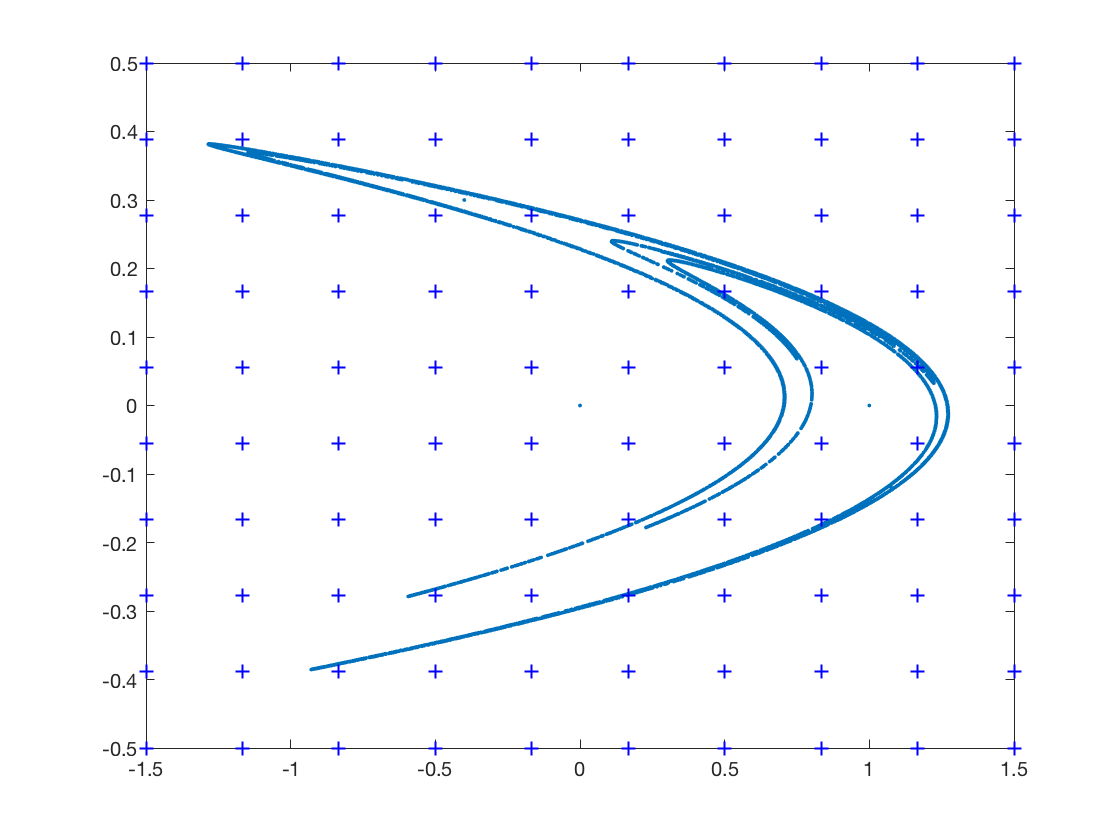
\includegraphics[width=\textwidth]{invarianthenon.png}
		\label{henon0}
	\end{subfigure}
	~ %add desired spacing between images, e. g. ~, \quad, \qquad, \hfill etc. 
	%(or a blank line to force the subfigure onto a new line)
	\begin{subfigure}[b]{0.4\textwidth}
		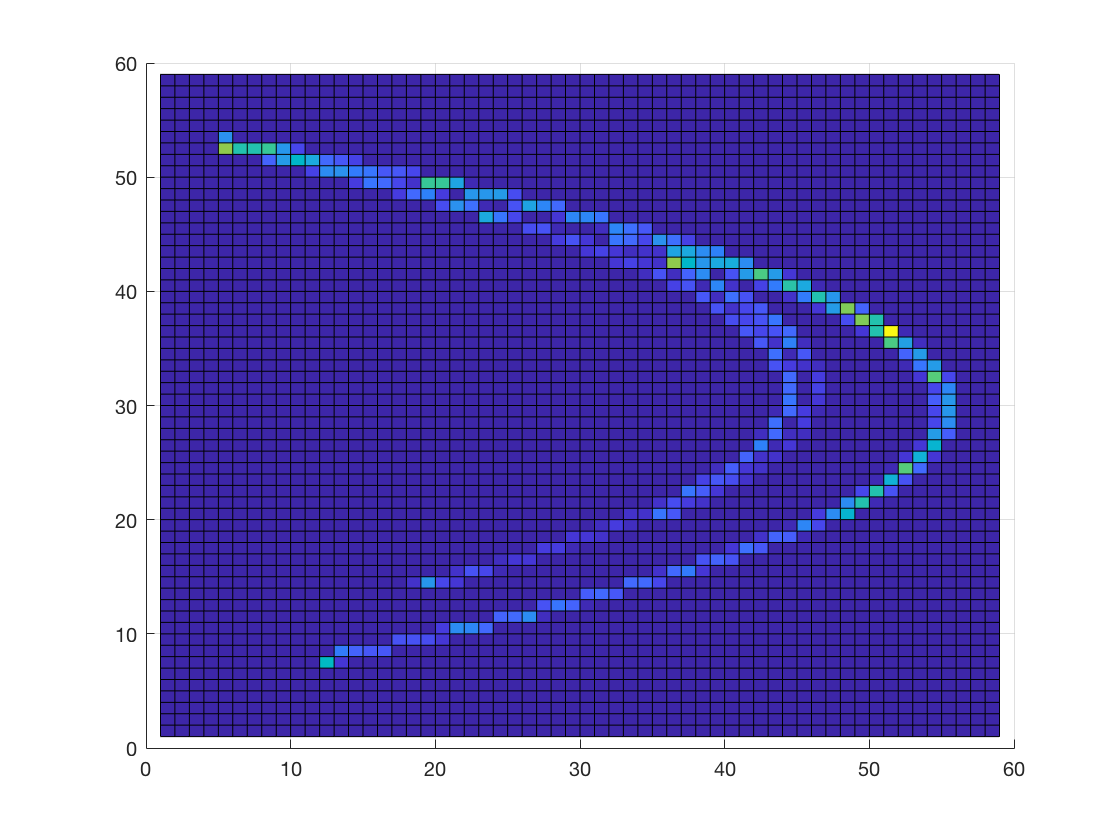
\includegraphics[width=\textwidth]{henonmap.png}
		\label{fig:tiger}
	\end{subfigure}
	 %add desired spacing between images, e. g. ~, \quad, \qquad, \hfill etc. 
	%(or a blank line to force the subfigure onto a new line)
	\caption{On the left we show the box discretisation of the phase space and a long run of the H\'{e}non map taking $[0,0]$ as the initial condition. On the right there is a plot of the normalised invariant measure of the system.}\label{Henon}
\end{figure}

The spectrum of the transition matrix is given in Figure PPP. We observe that there is a spectral gap. Of course, this just means that this approximation of the transfer operator can be iterated and it will eventually converge. We also present a rought estimate of the generator of the transfer semigroup. We observe that this approximation matches the theoretical results that tell us that the spectrum should be contained in the left-hand-side of the complex plane. This is a confirmation of Hille-Yoshida theorem, which establishes the conditions by which an operator generates a semigroup. To obtain this estimate one has to take the formal logarithm of the transition matrix.

\begin{figure}[H]
	\centering
	\begin{subfigure}[b]{0.4\textwidth}
		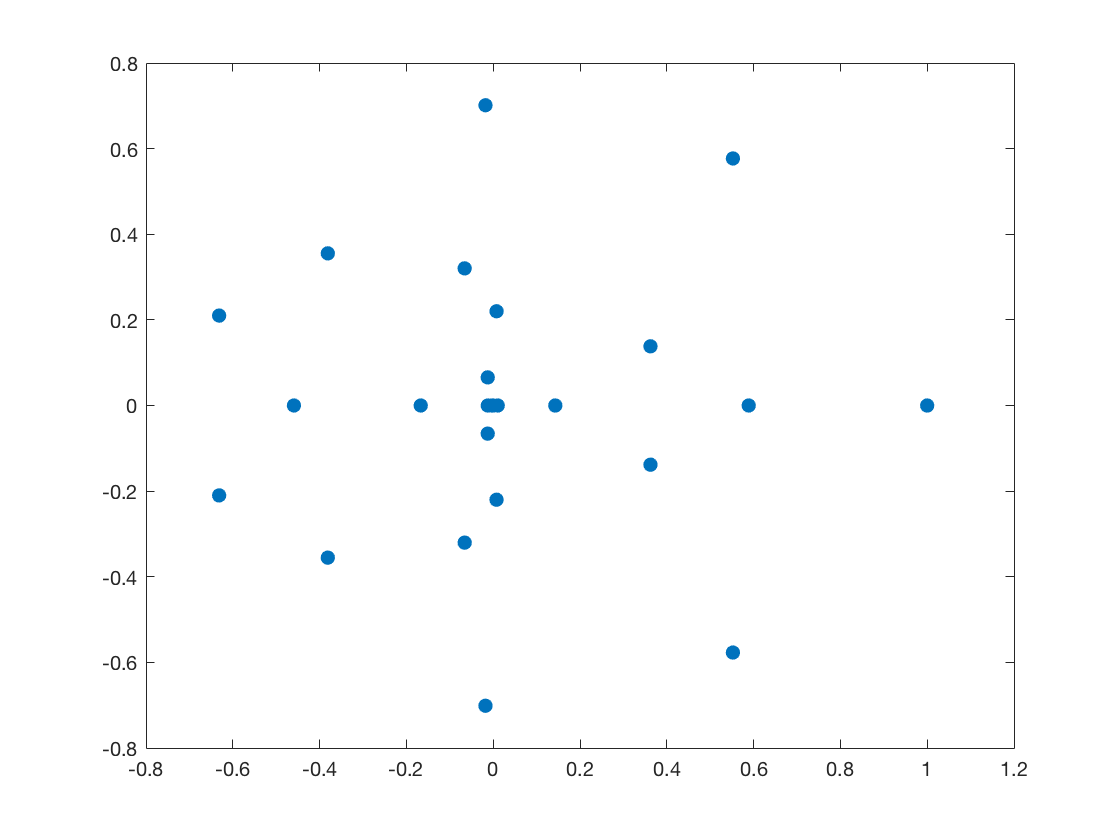
\includegraphics[width=\textwidth]{spectrumhenon.png}
		\label{henon0}
	\end{subfigure}
	~ %add desired spacing between images, e. g. ~, \quad, \qquad, \hfill etc. 
	%(or a blank line to force the subfigure onto a new line)
	\begin{subfigure}[b]{0.4\textwidth}
		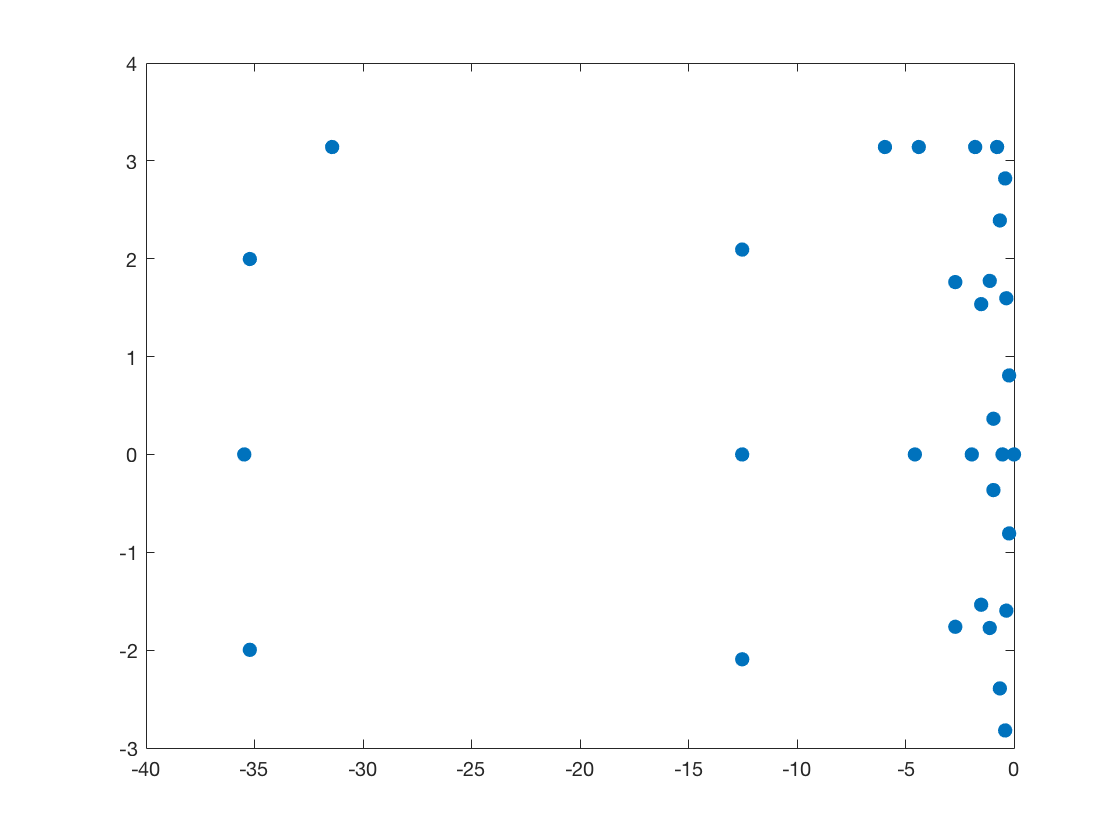
\includegraphics[width=\textwidth]{ruellepollicothenon.png}
		\label{fig:tiger}
	\end{subfigure}
	%add desired spacing between images, e. g. ~, \quad, \qquad, \hfill etc. 
	%(or a blank line to force the subfigure onto a new line)
	\caption{The first picture shows the spectrum of the transition matrix of the H\'{e}non map. The second corresponds to the spectrum of the logarithm of the transition matrix.}
\end{figure}

Following the study of discrete maps, we consider now a new Poincaré section of Lorenz' 84 model. To approximate the transfer operator we proceeded in the same way as before. By integrating the equations for long enough, we obtained a trajectory consisting of 649 points. To solve the equations numerically, we used the built-in Matlab command ode45. In Figure PPP we observe a realisation of a trajectory and the domain divided into boxes of size ?? along with the invariant measure of the system. 

\begin{figure}[H]
	\centering
	\begin{subfigure}[b]{0.4\textwidth}
		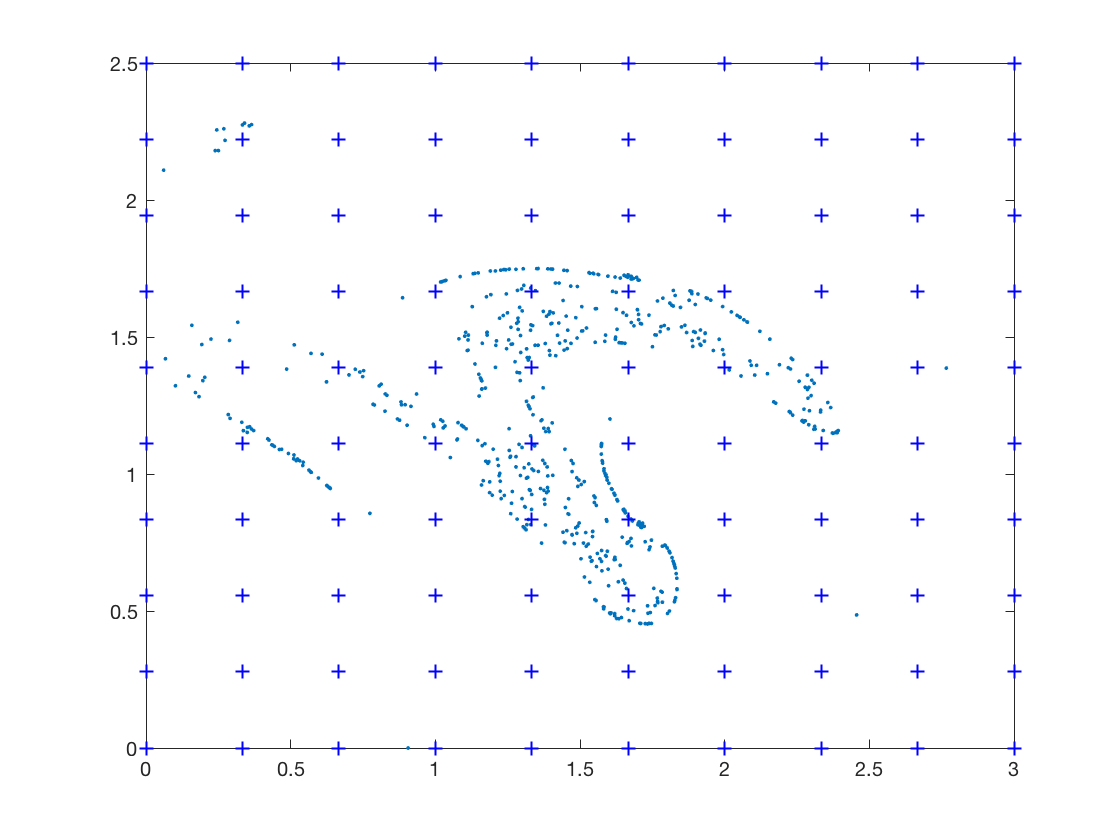
\includegraphics[width=\textwidth]{invariantl84.png}
		\label{henon0}
	\end{subfigure}
	~ %add desired spacing between images, e. g. ~, \quad, \qquad, \hfill etc. 
	%(or a blank line to force the subfigure onto a new line)
	\begin{subfigure}[b]{0.4\textwidth}
		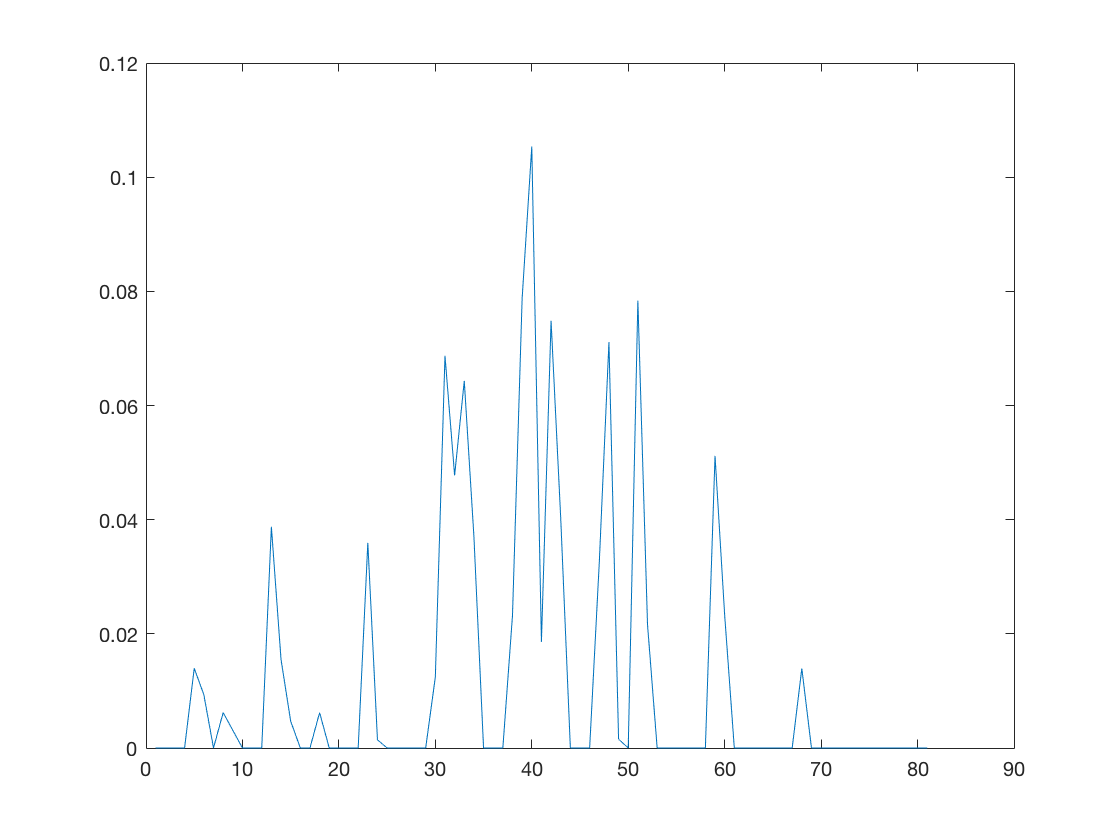
\includegraphics[width=\textwidth]{poincarel84map.png}
		\label{fig:tiger}
	\end{subfigure}
	%add desired spacing between images, e. g. ~, \quad, \qquad, \hfill etc. 
	%(or a blank line to force the subfigure onto a new line)
	\caption{Normalised invariant density (right) and sample trajectory of the Poincar\'{e} section of Lorenz' 84 (left).}
\end{figure}

The spectrum of the transition matrix computed for this discrete map shows, as in the previous case that this approximation has a spectral gap and therefore matrix power iterations will lead to exponentially fast convergence. We highlight that this does not show that the map is actually exponentially mixing.

\begin{figure}[H]
	\centering
	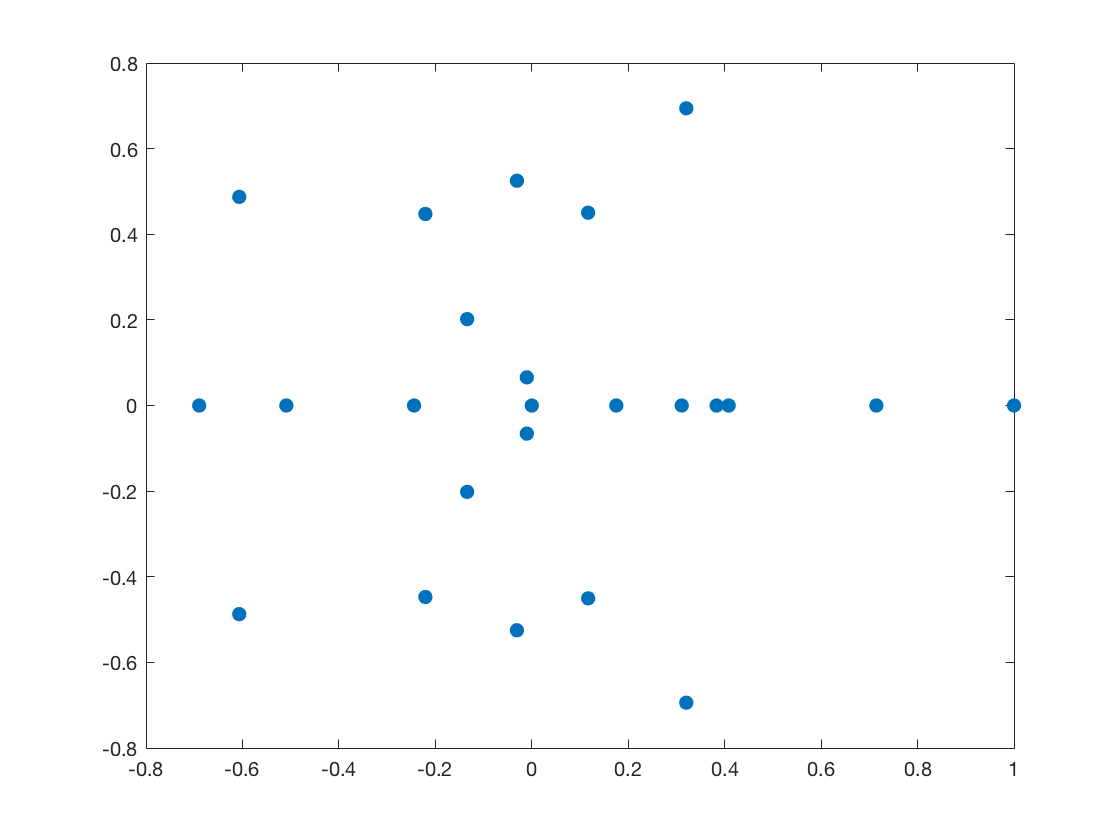
\includegraphics[scale=0.2]{spectruml84.png}
	\caption{Spectrum of the transition matrix of the Poincar\'{e} section of Lorenz 84.}
\end{figure}

To imiplement Ulam's method for continuous dynamical systems we have used the Matlab package GAIO REFERENCE. This package provides efficient tools to calculate the phase space discretisation and to obtain approximations of the unstable manifold of the system amongst other features. In this document, we present some experiments done using GAIO to calculate a box discretisation of the phase space and the calculation of the invariant measure of the system.

 Unlike the previous examples, the algorithm presented by GAIO does not run a long integration of the model and wait enough time to populate the attractor. Rather, GAIO provides two different ways of computing the transition matrix, namely, computation by \emph{test-points} or computation by \emph{exhaustion}. Using test-points method to compute the transition matrix consists of taking sample points within each box of the discretisation of the phase space and examining where they move after an interation of the flow. These test points can be randomly chosen so often these points are called Monte Carlo points REF. The exhaustion method works as follows. Consider the boxes $A$ and $B$, so that we want to estimate the volume of $A\cap T^{-1}(B)$. First, we subdived a box $A$ into smaller ones of the same size. Second, we test wether the forward image of some of the smaller boxes within $A$ fit into $B$. If the image does not fit, we reduced the size of the subdivision of $A$. This idea mimics the exhaustion method that can be found in The Elements.

As an experiment we considered Lonrez' 63 model. First of all we calculate the flow of the system, which is given by the solution of the equation. These experiments are motivated by \cite{lucarini} where similar experiments are performed. The aim is to calculate the response of the system in a finite state Markov chain framework with a transfer operator approach. We note that the procedure we present is different  On one hand, in \cite{lucarini} we observe that a long integration of the equations is done where as here the flow is symbolically approximated using an explicit fourth order Runge-Kutta algorithm as we show below:

\begin{verbatim}
	function X = rk4(v,X,h,n)
	
	% RK4   Fourth order Runge-Kutta algorithm 
	% performs n steps of the scheme for the vector field v
	% using stepsize h on each row of the matrix X
	% v maps an (m x d)-matrix to an (m x d)-matrix 
	
	    for i = 1:n
	        k1 = v(X);
	        k2 = v(X + h/2*k1);
	        k3 = v(X + h/2*k2);
	        k4 = v(X + h*k3);
	        X = X + h*(k1 + 2*k2 + 2*k3 + k4)/6;
	    end
\end{verbatim}
Secondly, this form of the flow is used to calculate the transition matrix as described in the test-points method, different to that done in \cite{lucarini}. In Figure ??? we observe several outputs of the box covering of the attractor of Lorenz 63 model using GAIO for different resolutions. The command used for the plot is called \texttt{boxplot3()}. Although we have not gone into the details, this algorithm also approximates the unstable manifold of the system. It is remarkable that 20 seconds are needed to do a box covering of 33320 microstates.  

\begin{figure}[H]
	\centering
	\begin{subfigure}[b]{0.4\textwidth}
		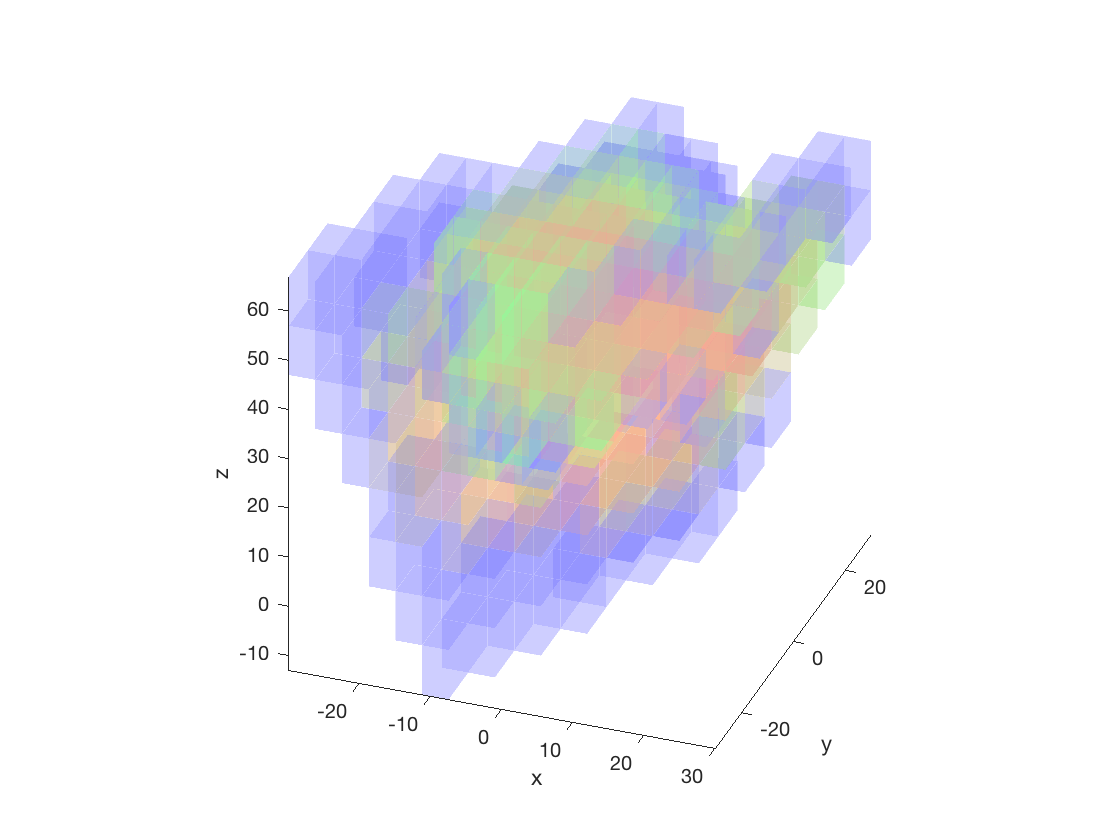
\includegraphics[width=\textwidth]{l63n10.png}
		\caption{342 microstates or boxes.}
		\label{l63n10}
	\end{subfigure}
	~ %add desired spacing between images, e. g. ~, \quad, \qquad, \hfill etc. 
	%(or a blank line to force the subfigure onto a new line)
	\begin{subfigure}[b]{0.4\textwidth}
		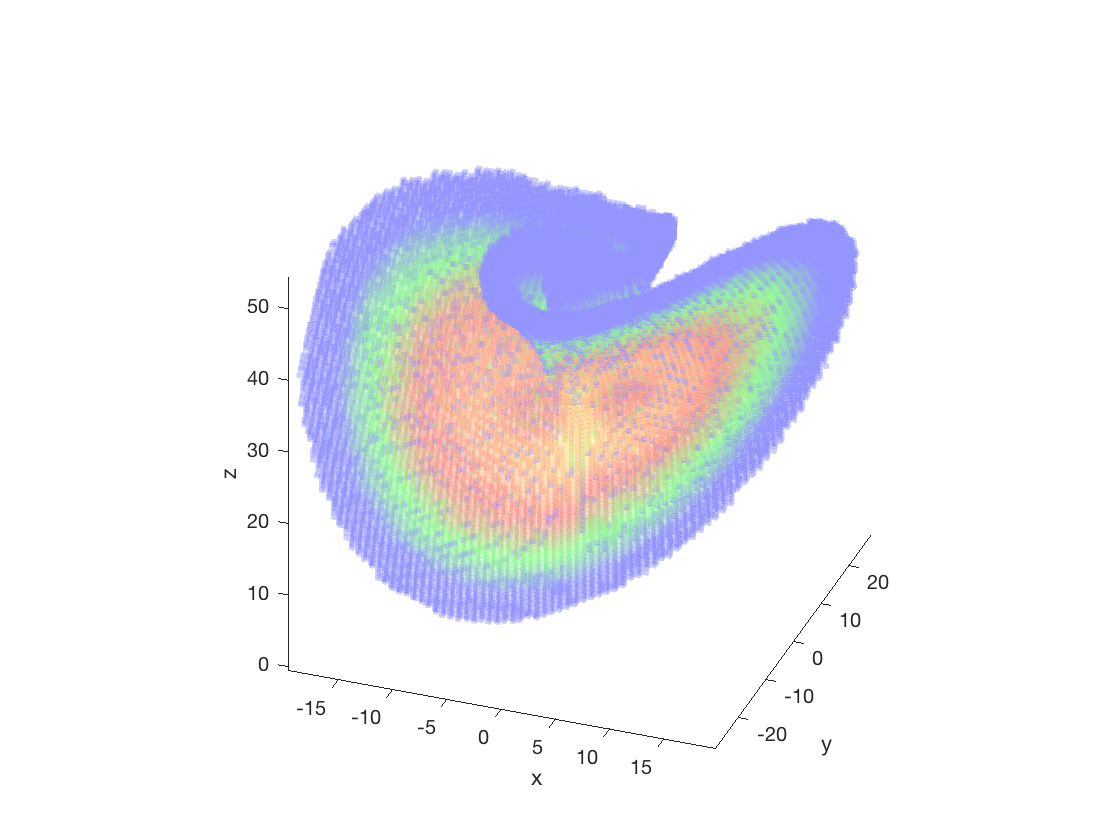
\includegraphics[width=\textwidth]{l63n21.png}
		\caption{33320 microstates or boxes.}
	\end{subfigure}
	\caption{Output of GAIO for the box covering of the Lorenz 63 attractor. The red colour indicates the highly populated parts of the attractor.}
\end{figure}

The existence of a spectral gap in Lorenz 63 model is not apparent from the calculated approximations. For low resolutions, the approximate spectral gap fluctuates to eventually decay in a very slow way (see Figure \ref{sp}).

\begin{figure}[H]
	\centering
	\begin{subfigure}[b]{0.4\textwidth}
		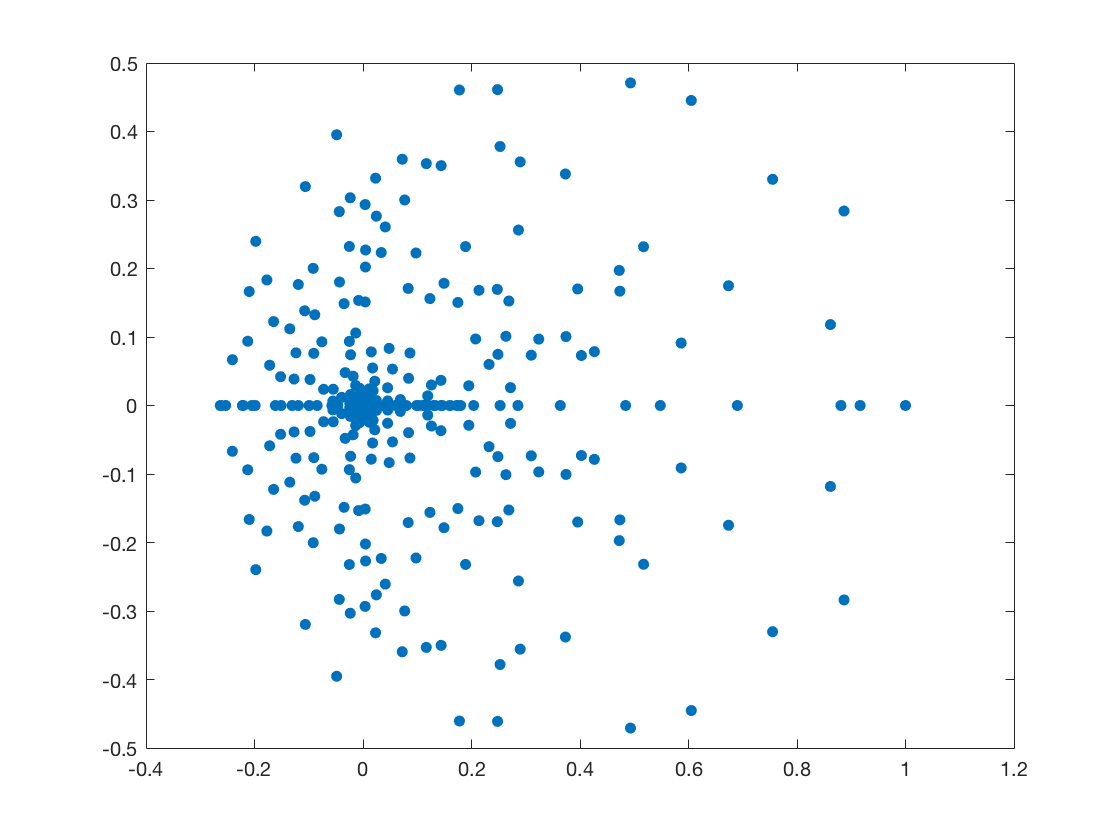
\includegraphics[width=\textwidth]{spectruml63.png}
	\end{subfigure}
	~ %add desired spacing between images, e. g. ~, \quad, \qquad, \hfill etc. 
	%(or a blank line to force the subfigure onto a new line)
	\begin{subfigure}[b]{0.4\textwidth}
		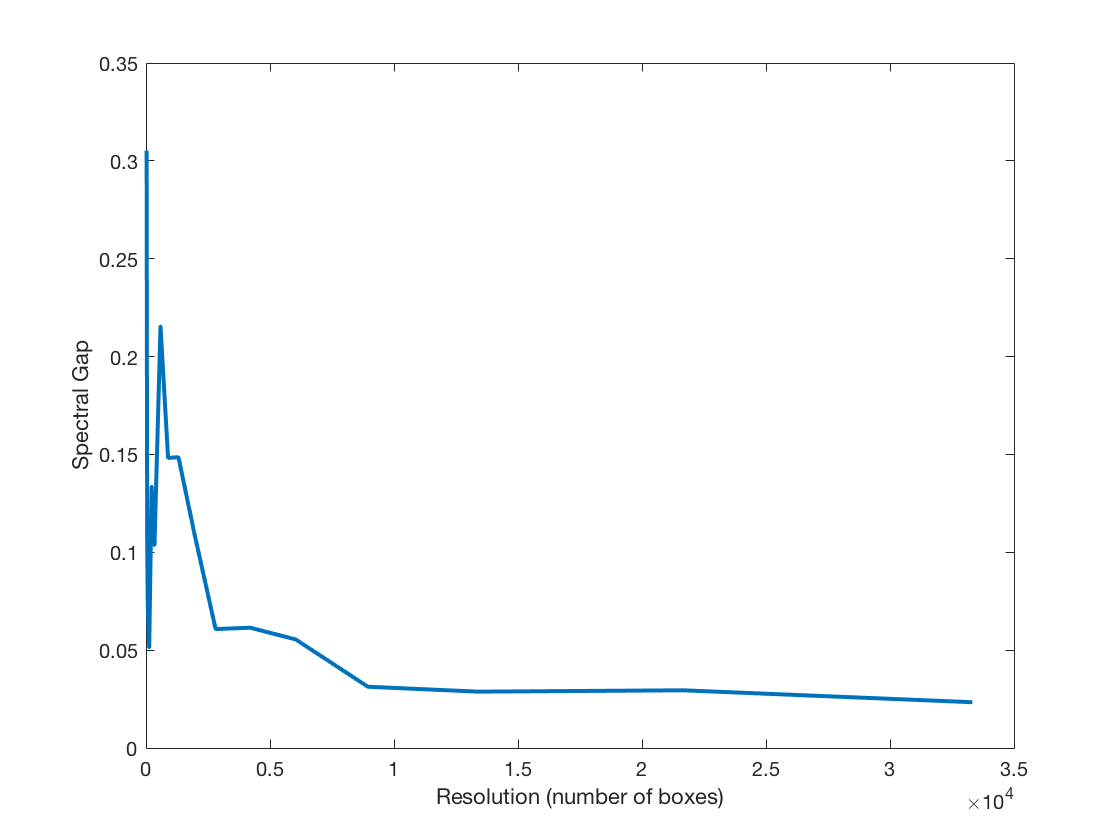
\includegraphics[width=\textwidth]{spectralgapl63.png}
	\end{subfigure}
	\caption{\label{sp} To the left, subset of the complex plane containing the approximate spectrum of the transfer operator of Lorenz 63 for a resolution of 2800 boxes. On the right, the evolution of the spectral gap of the system as a function of the resolution considered.}
\end{figure}
As commented earlier in the text, the invariant measure of the system is obtained by solving the eigenvalue problem for the eigenvalue $1$. Computationally, however, it is not trivial to solve the eigenvalue problem, especially if one deals with matrices with 33320$^2$ entries (8.3GB). It is the case that these Markov matrices are sparse and thus we have to manipulate these matrices in sparse mode. Matlab command \texttt{eigs(M,k)} allows us to, iteratively, compute the \texttt{k} largest eigenvalues of the Matrix. In particular for the calculation of the eigenvector associated with the largest eigenvalue ($1$), we take \texttt{k}=1 and \texttt{k}=2 when considering the spectral gap.



L63
L84

\section*{Future Work}

The theory concerning Markov operators and their relevance in response theory is that has to be studied in the next stage. The spectral properties of the Markov operators describing the evolution of densities in a system is far from trivial and they can change depending on the system we are dealing with. Also, the well-posedness of response theory for certain dynamical system is an open problem. We shall carry on constructing a background in this topic by reading the results of LIVERANI MAJDA HAIRER BALADI.

The software GAIO uses a set of algorithms that are efficient but not obvious. A deeper understanding of GAIO, particularly of the \texttt{Tree} Matlab class REF, is needed to be able to extract more dynamical information. Using this package, we will continue to reproduce the results in \cite{lucarini} and try to calculate the nonlinear terms in the response operator mentioned, also for the observables $x^2$, $y^2$, $z^2$ and $z$.

It is specially relevant in climate to consider non-infinitesimal perturbations of the system, it is here where it is very relevant to be able to compute the nonlinear terms of the response. REWVIEW

Further, the transfer operators (in general, Markov models) are also a technique used to identify invariant and quasi-invariant sets. This has a wide scope of application when it comes to identifying quasi-invariant sets as suggested in LETTER, where they use a transfer 

The numerical experi


